%%%%%%%%%%%%%%%%%%%%%%%%%%%%%%%%%%%%%%%%%%%%%%%%%%%%%%%%
%%%%%%%%%%%%%%%%%%%%%%%%%%%%%%%%%%%%%%%%%%%%%%%%%%%%%%%%
%%%                                                  %%%
%%% University of Arizona themed Beamer presentation %%%
%%% Based on the Warsaw, Palo Alto and UNL templates %%%
%%% modified by Joseph V. Casillas (6-13-2011)       %%%
%%%                                                  %%%
%%%%%%%%%%%%%%%%%%%%%%%%%%%%%%%%%%%%%%%%%%%%%%%%%%%%%%%%
%%%%%%%%%%%%%%%%%%%%%%%%%%%%%%%%%%%%%%%%%%%%%%%%%%%%%%%%

\documentclass{beamer}
\mode<presentation>{\usetheme{UA2}\setbeamercovered{transparent}}
\usepackage[english]{babel}
\usepackage[utf8]{inputenc}
\usepackage{t1enc}
\usepackage{verbatim}
\usepackage{media9}
\usepackage{apacite}
\usepackage{tipa}
\usepackage{amssymb}   
\usepackage{soul}               % \hl{highlight this text}
\usepackage{graphicx}           % Put .eps and .pdf images into document
\usepackage{colortbl}
\usepackage{times}
\usepackage{url}				%this allows us to cite URLs in the text
\usepackage{qtree}
\usepackage{pifont}
\newcommand{\cmark}{\ding{51}}%
\newcommand{\xmark}{\ding{55}}%

\title[Acoustics of coronal stops]{Acoustics of coronal stops in \\ Spanish-English bilingual speech}
\author[Casillas, D\'{i}az \& Simonet, 2015]{\textbf{Joseph V. Casillas}, \textbf{Yamile D\'{i}az} \& \textbf{Miquel Simonet} \\ University of Arizona, Tucson}
\date{Dep. of Spanish \& Portuguese \\ February, 2016 | Tucson, Arizona \\ University of Arizona}

\begin{document}

\begin{frame}
  \titlepage
\end{frame}

\section{Introduction} % (fold)
\label{sec:introduction}

\subsection{Spanish and English}

\begin{frame}
\frametitle{Overview}
\begin{itemize}
	\item Spanish and English both have \textipa{/d/} and \textipa{/t/}
	\item Phonetic descriptions differ as a function of language
	\begin{itemize}
		\item Spanish \textipa{/d t/} described as dental
		\item English \textipa{/d t/} described as alveolar
	\end{itemize}
	\item Present study is concerned with:
	\begin{itemize}
		\item description of acoustics of \textipa{/d t/} at release
		\item comparisons of monolinguals and bilinguals
		\item comparisons of two languages of a bilingual
	\end{itemize}
\end{itemize}
\end{frame}

\begin{frame}
\frametitle{Introduction}
\begin{itemize}
	\item Spanish and English contrast between \textipa{/p t k/} and \textipa{/b d g/}
	\item The phonetics of `voicing' in stop differs
	\begin{itemize}
		\item Spanish \textipa{/d/} is prevoiced and \textipa{/t/} is voiceless
		\item English \textipa{/d/} is voiceless and \textipa{/t/} is aspirated
	\end{itemize}
\end{itemize}
\begin{center}
	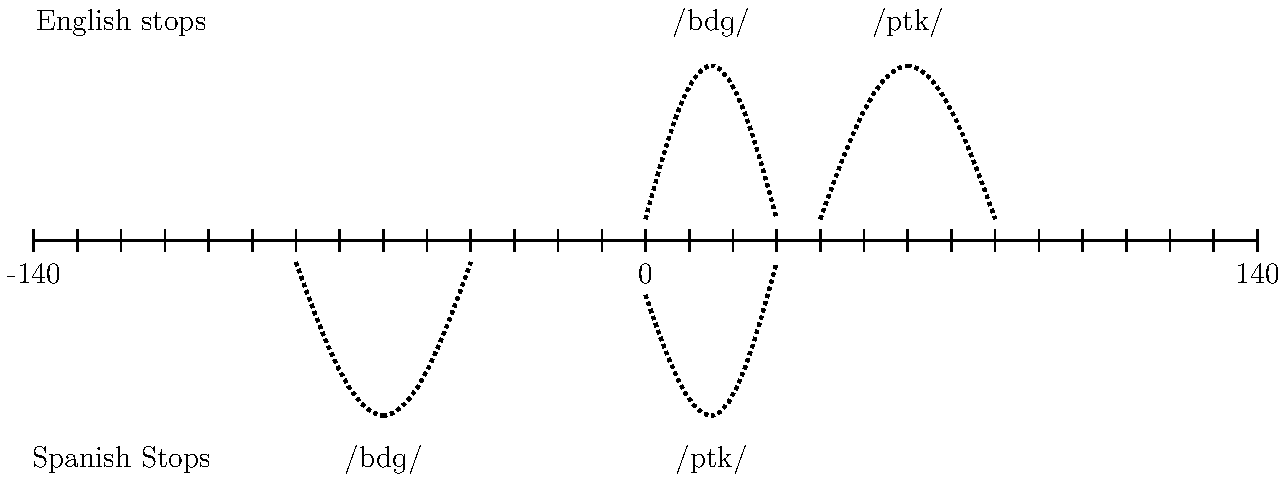
\includegraphics[width=.7\textwidth]{figures/sp_en_stops.pdf}
\end{center}
\end{frame}


\begin{frame}
\frametitle{Introduction}
\begin{itemize}
	\item Spanish and English coronal stops (\textipa{/d t/}) also differ in \textbf{place of articulation}
	\begin{itemize}
		\item Spanish \textipa{/d/} and \textipa{/t/} are described as dental
		\item English \textipa{/d/} and \textipa{/t/} are described as alveolar
	\end{itemize}
	\item Some articulatory data are available
	\item \textbf{How is this reflected on the acoustic signal?}
\end{itemize}
\end{frame}

\subsection{Coronal stops}

\begin{frame}
\frametitle{Introduction}
\begin{itemize}
	\item Jongman et al. (1985) \begin{itemize} \item for Malayalam, which contrasts dental and alveolar stops, and Dutch (dental) vs. English (alveolar) stops \end{itemize}
	\item Stoel-Gamon et al. (1994) \begin{itemize} \item for Swedish (dental) vs. English (alveolar) stops \end{itemize}
	\item Sundara (2005, 2006) \begin{itemize} \item for Canadian French and Canadian English \\ and French-English bilinguals \end{itemize}
\end{itemize}
\end{frame}

\begin{frame}
\frametitle{Introduction}
\begin{itemize}
	\item At release burst, alveolar stops are louder than dental stops (relative amplitude, intensity)\footnote{Jongman et al., 1985; Stoel-Gamon et al., 1994; Sundara, 2005, 2006}
	\item Spectral envelope of burst captures differences between alveolar and dental stops\footnote{Stoel-Gamon et al., 1994; Sundara, 2005, 2006}
	\begin{itemize}
		\item center of gravity of spectrum, higher for alveolars
		\item standard deviation of spectrum, more compact for alveolars
		\item kurtosis of spectrum, more peaked for alveolars
	\end{itemize}
\end{itemize}
\end{frame}

\begin{frame}
\frametitle{Introduction}
\begin{itemize}
	\item Malayalam, which contrasts alveolars and dentals, uses `strict' acoustic correlates for both consonant types; i.e., there is little overlap between acoustic distributions\footnote{Jongman, 1985}
	\item Languages tend to have \emph{either} dental \emph{or} alveolar; i.e., few languages contrast dentals and alveolars
	\item In languages with no contrast, acoustic correlates are more variable, flexible (leading to more overlap)
	\begin{itemize}
		\item \alert{what happens in bilingualism?}
		\item \alert{one individual = dental $+$ alveolar}
	\end{itemize}
\end{itemize}
\end{frame}

\subsection{Bilingual speech}

\begin{frame}
\frametitle{Introduction}
\begin{itemize}
	\item In bilingualism, links are formed between sound categories in the two languages
	\item Interlingual links lead to assimilations, compromise
	\item Caramazza et al., 1973:
	\begin{itemize}
		\item French-English bilinguals in Montr\'{e}al, Qu\'{e}bec
		\item bilinguals use VOT differently in their two languages
		\item but values `compromised' between two languages
	\end{itemize}
	\item \alert{Bilinguals with dental and alveolar stops might compromise their place of articulation for [coronal] stops}
	\begin{itemize}
		\item articulatory difference is small
		\item acoustic difference is unstable
	\end{itemize}
\end{itemize}
\end{frame}

\begin{frame}
\frametitle{Introduction}
\begin{itemize}
	\item Sundara, 2006 (simultaneous bilinguals)
	\begin{itemize}
		\item French-English bilinguals in Montr\'{e}al, Qu\'{e}bec
		\item French \textipa{/d t/} (dental) vs. English \textipa{/d t/} (alveolar)
		\item Bilinguals keep languages separate, but they also differ from monolinguals (acoustic correlates not fully distinctive)
	\end{itemize}

\end{itemize}
\end{frame}

\begin{frame}
\frametitle{Introduction}
\begin{itemize}
	\item Some early and simultaneous bilinguals use language-specific phonetics consistently
	\item Bilinguals might have separate phonetic (sub)systems
	\item Magloire and Green, 1999:
	\begin{itemize}
		\item early Spanish-English bilinguals from Arizona
		\item recruited in unilingual sessions (Spanish, English)
		\item in production of VOT categories, bilinguals did not differ from monolinguals in any language and any condition
	\end{itemize}
	\item \textbf{Perhaps this population allows for the study of dental-alveolar place in within-subjects design}
\end{itemize}
\end{frame}


\section{Method} % (fold)
\label{sec:method}
\subsection{Speakers}

\frame{\begin{center} \textbf{METHOD} \\ speakers | materials | analyses \end{center}}

\frame{\frametitle{Participants}
\begin{itemize}
	\item \textbf{32 participants, all of them females}
	\begin{itemize}
		\item 8 Spanish-speaking monolinguals from Majorca, Spain
		\item 8 English-speaking monolinguals from Tucson, Arizona
		\item 16 Spanish-English bilinguals from Tucson, Arizona
		\begin{itemize}
			\item 8 dominant in Spanish
			\item 8 dominant in English
    		\end{itemize}
 	\end{itemize}
  	\item Young adults: ages 18--25
  	\item \textbf{Bilingual Language Profile \{BLP\} questionnaire}\footnote{Birdsong, Amengual, Gertken, 2012}
  \end{itemize}}

\frame{\frametitle{Participants}
\begin{itemize}
  	\item \textbf{Bilingual Language Profile} has four components:
  	\begin{itemize}
    		\item history (6 questions)
    		\item use (5 questions)
    		\item competency (4 questions)
    		\item attitudes (4 questions)
	\end{itemize}
 	\item Responses are numeric\footnote{age of learning, years of use, percentages of use, Likert-type scales, etc.}
  	\begin{itemize}
    		\item score assigned to each language
    		\item dominance score obtained by subtraction (-218 to 218)
    		\begin{itemize}
    			\item Negative values = dominant in English (\emph{M} = \textbf{-33.37})
    			\item Positive values = dominant in Spanish (\emph{M} = \textbf{30})
    		\end{itemize}
  	\end{itemize}
\end{itemize}}

\subsection{Materials}

\begin{frame}
\frametitle{Materials}
\begin{itemize}
	\item words with \textipa{/d/} or \textipa{/t/} in utterance-initial position
	\item words in carrier sentence
	\begin{itemize}
		\item `\emph{tanto} es la palabra'
		\item `\emph{tantrum} is the word'
	\end{itemize}
	\item lexical stress, controlled (stressed, prestressed)
	\item first vowel, controlled (always low: \textipa{/a/} or \textipa{/\ae/})
	\begin{itemize}
		\item Spanish: \emph{danza} (12), \emph{tanto} (12)
		\item English: \emph{dancing} (12), \emph{tantrum} (12)
	\end{itemize}
\end{itemize}
\end{frame}

\begin{frame}
\frametitle{Procedure}
\begin{itemize}
	\item \textbf{Delayed shadowing technique}
	\begin{itemize}
		\item auditory stimuli: male speech
		\item six male ``talkers'' (3 Spanish, 3 English) recorded stimuli
		\item stimuli played in random order to the speakers\footnote{`talkers' were monolinguals from Spain (Spanish) or Texas (English)}
		\item speakers ``listened and repeated sentences''
	\end{itemize}
	\item \textbf{Who produced what?}
	\begin{itemize}
		\item Spanish monolinguals, only Spanish materials
		\item English monolinguals, only English materials
		\item Spanish-English bilinguals, both languages
		\begin{itemize}
			\item both languages in one block
			\item random order
		\end{itemize}
	\end{itemize}
\end{itemize}
\end{frame}

\subsection{Analyses}

\begin{frame}
\frametitle{Data}
\begin{itemize}
	\item \textbf{24} (words) $\times$ \textbf{3} (iterations) $\times$ \textbf{2} (languages)
	\begin{itemize}
		\item 576 tokens, Spanish monolinguals
		\item 576 tokens, English bilinguals
		\item 1152 tokens, Spanish-dominant bilinguals
		\item 1152 tokens, English-dominant bilinguals
	\end{itemize}
	\item Total: 3,456 (- 76 errors) = \textbf{3380} tokens in dataset
\end{itemize}
\end{frame}

\begin{frame}
\frametitle{Acoustic analyses}
\begin{itemize}
	\item \textbf{Voice Onset Times (ms)}
	\begin{itemize}
		\item onset of burst minus onset of modal voicing
		\item from negative (lead VOT) to positive (long-lag VOT)
	\end{itemize}
	\item \textbf{Gaussian window left-aligned with burst onset}
	\begin{itemize}
		\item if VOT positive, but less than 20 ms, \\ analysis window equals VOT
		\item if VOT positive, but more than 20m, \\analysis window equals 20 ms
		\item if VOT negative, \\analysis window equals 20 ms
	\end{itemize}
	\item \textbf{Power spectrum from gaussian window}
\end{itemize}
\end{frame}

\begin{frame}
\frametitle{Acoustic analyses}
\begin{itemize}
	\item \textbf{VOTs (ms)}
	\item \textbf{Spectral characteristics of burst}
	\begin{itemize}
		\item Center of Gravity (Hz)
		\item Standard Deviation
		\item Skewness
		\item Kurtosis
	\end{itemize}
	\item \textbf{Relative burst intensity}
	\begin{itemize}
		\item Intensity of burst (dB) minus intensity at vowel midpoint
	\end{itemize}
\end{itemize}
\end{frame}

\begin{frame}
\frametitle{Acoustic analyses}
\begin{itemize}
	\item \textbf{\alert{VOTs (ms)}}
	\item \textbf{\alert{Spectral characteristics of burst}}
	\begin{itemize}
		\item \alert{Center of Gravity (Hz)}
		\item Standard Deviation
		\item Skewness
		\item Kurtosis
	\end{itemize}
	\item \textbf{\alert{Relative burst intensity}}
	\begin{itemize}
		\item Intensity of burst (dB) minus intensity at vowel midpoint
	\end{itemize}
\end{itemize}
\end{frame}

\begin{frame}
\frametitle{Statistical analyses}
\begin{itemize}
	\item Linear mixed-effects regression
	\item Here, by-subject (mixed-design) ANOVAs
	\begin{itemize}
		\item response: VOT, COG, RI separately
		\item factors: language (2), voicing (2), group (4)
	\end{itemize}
\end{itemize}
\end{frame}

\begin{frame}
\frametitle{Statistical analyses}
\begin{itemize}
	\item How do English and Spanish /d t/ differ?
	\begin{itemize}
		\item only monolingual productions
		\item 2 (voicing) $\times$ 2 (language) $\times$ 2 (group)
	\end{itemize}
	\item How do monolinguals and bilinguals differ?
	\begin{itemize}
		\item only Spanish productions
		\item 2 (voicing) $\times$ 3 (group)
	\end{itemize}
	\item How do monolinguals and bilinguals differ?
	\begin{itemize}
		\item only English productions
		\item 2 (voicing) $\times$ 3 (group)
	\end{itemize}
	\item How do the two languages of a bilingual differ?
	\begin{itemize}
		\item only bilingual productions
		\item 2 (voicing) $\times$ 2 (language) $\times$ 2 (group)
	\end{itemize}
\end{itemize}
\end{frame}

\begin{frame}
\frametitle{Statistical analyses}
\begin{itemize}
	\item \textbf{How do English and Spanish /d t/ differ?}
	\begin{itemize}
		\item only monolingual productions
		\item 2 (voicing) $\times$ 2 (language) $\times$ 2 (group)
	\end{itemize}
	\item How do monolinguals and bilinguals differ?
	\begin{itemize}
		\item only Spanish productions
		\item 2 (voicing) $\times$ 3 (group)
	\end{itemize}
	\item How do monolinguals and bilinguals differ?
	\begin{itemize}
		\item only English productions
		\item 2 (voicing) $\times$ 3 (group)
	\end{itemize}
	\item How do the two languages of a bilingual differ?
	\begin{itemize}
		\item only bilingual productions
		\item 2 (voicing) $\times$ 2 (language) $\times$ 2 (group)
	\end{itemize}
\end{itemize}
\end{frame}

\begin{frame}
\frametitle{Statistical analyses}
\begin{itemize}
	\item How do English and Spanish /d t/ differ?
	\begin{itemize}
		\item only monolingual productions
		\item 2 (voicing) $\times$ 2 (language) $\times$ 2 (group)
	\end{itemize}
	\item \textbf{How do monolinguals and bilinguals differ?}
	\begin{itemize}
		\item only Spanish productions
		\item 2 (voicing) $\times$ 3 (group)
	\end{itemize}
	\item How do monolinguals and bilinguals differ?
	\begin{itemize}
		\item only English productions
		\item 2 (voicing) $\times$ 3 (group)
	\end{itemize}
	\item How do the two languages of a bilingual differ?
	\begin{itemize}
		\item only bilingual productions
		\item 2 (voicing) $\times$ 2 (language) $\times$ 2 (group)
	\end{itemize}
\end{itemize}
\end{frame}

\begin{frame}
\frametitle{Statistical analyses}
\begin{itemize}
	\item How do English and Spanish /d t/ differ?
	\begin{itemize}
		\item only monolingual productions
		\item 2 (voicing) $\times$ 2 (language) $\times$ 2 (group)
	\end{itemize}
	\item How do monolinguals and bilinguals differ?
	\begin{itemize}
		\item only Spanish productions
		\item 2 (voicing) $\times$ 3 (group)
	\end{itemize}
	\item \textbf{How do monolinguals and bilinguals differ?}
	\begin{itemize}
		\item only English productions
		\item 2 (voicing) $\times$ 3 (group)
	\end{itemize}
	\item How do the two languages of a bilingual differ?
	\begin{itemize}
		\item only bilingual productions
		\item 2 (voicing) $\times$ 2 (language) $\times$ 2 (group)
	\end{itemize}
\end{itemize}
\end{frame}

\begin{frame}
\frametitle{Statistical analyses}
\begin{itemize}
	\item How do English and Spanish /d t/ differ?
	\begin{itemize}
		\item only monolingual productions
		\item 2 (voicing) $\times$ 2 (language) $\times$ 2 (group)
	\end{itemize}
	\item How do monolinguals and bilinguals differ?
	\begin{itemize}
		\item only Spanish productions
		\item 2 (voicing) $\times$ 3 (group)
	\end{itemize}
	\item How do monolinguals and bilinguals differ?
	\begin{itemize}
		\item only English productions
		\item 2 (voicing) $\times$ 3 (group)
	\end{itemize}
	\item \textbf{How do the two languages of a bilingual differ?}
	\begin{itemize}
		\item only bilingual productions
		\item 2 (voicing) $\times$ 2 (language) $\times$ 2 (group)
	\end{itemize}
\end{itemize}
\end{frame}


\section{Results} % (fold)
\label{sec:results}

\frame{\begin{center} \textbf{RESULTS} \\ study 1 | study 2 | study 3 | study 4 \end{center}}

\subsection{Study 1: Spanish vs. English \textipa{/d t/} in monolinguals}

\frame{\begin{center} \textbf{study 1} \\ Spanish \emph{vs.} English \textipa{/d t/} in monolinguals \end{center}}

\begin{frame}
\frametitle{Voice Onset Times (ms)}
\begin{center}
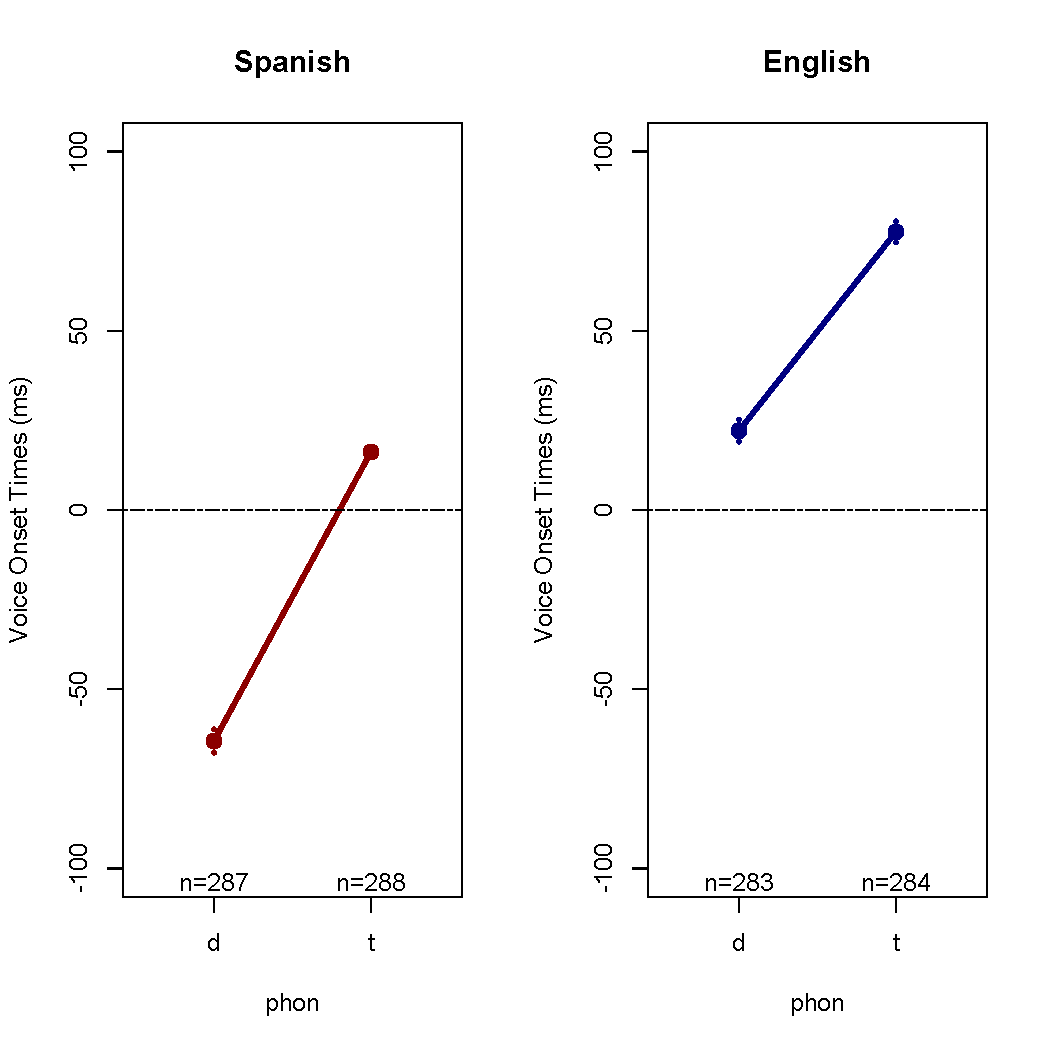
\includegraphics[scale=.375]{simplified/fig01_votmonolinguals.pdf}
\end{center}
\end{frame}

\begin{frame}
\frametitle{Center of Gravity (Hz)}
\begin{center}
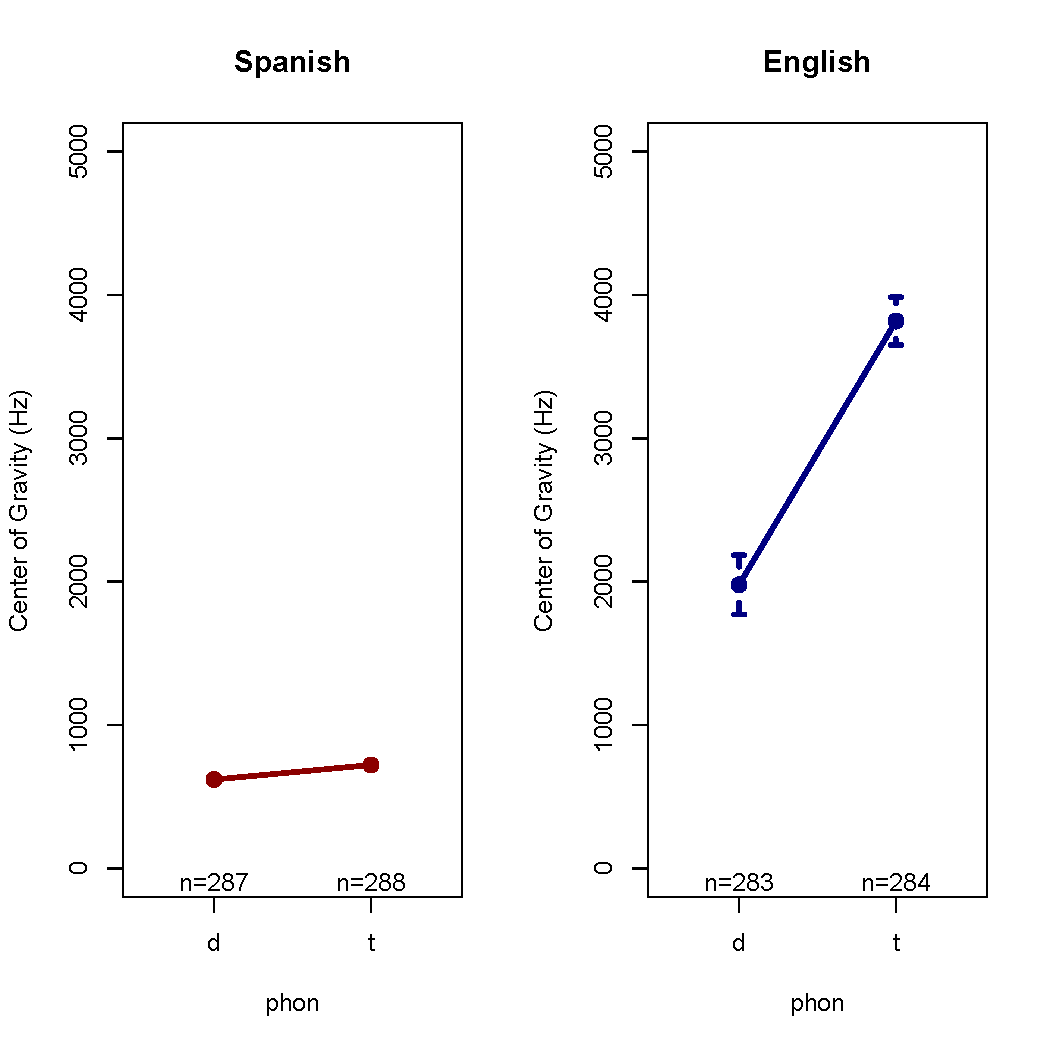
\includegraphics[scale=.375]{simplified/fig02_cogmonolinguals.pdf}
\end{center}
\end{frame}

\begin{frame}
\frametitle{Relative Intensity (dB)}
\begin{center}
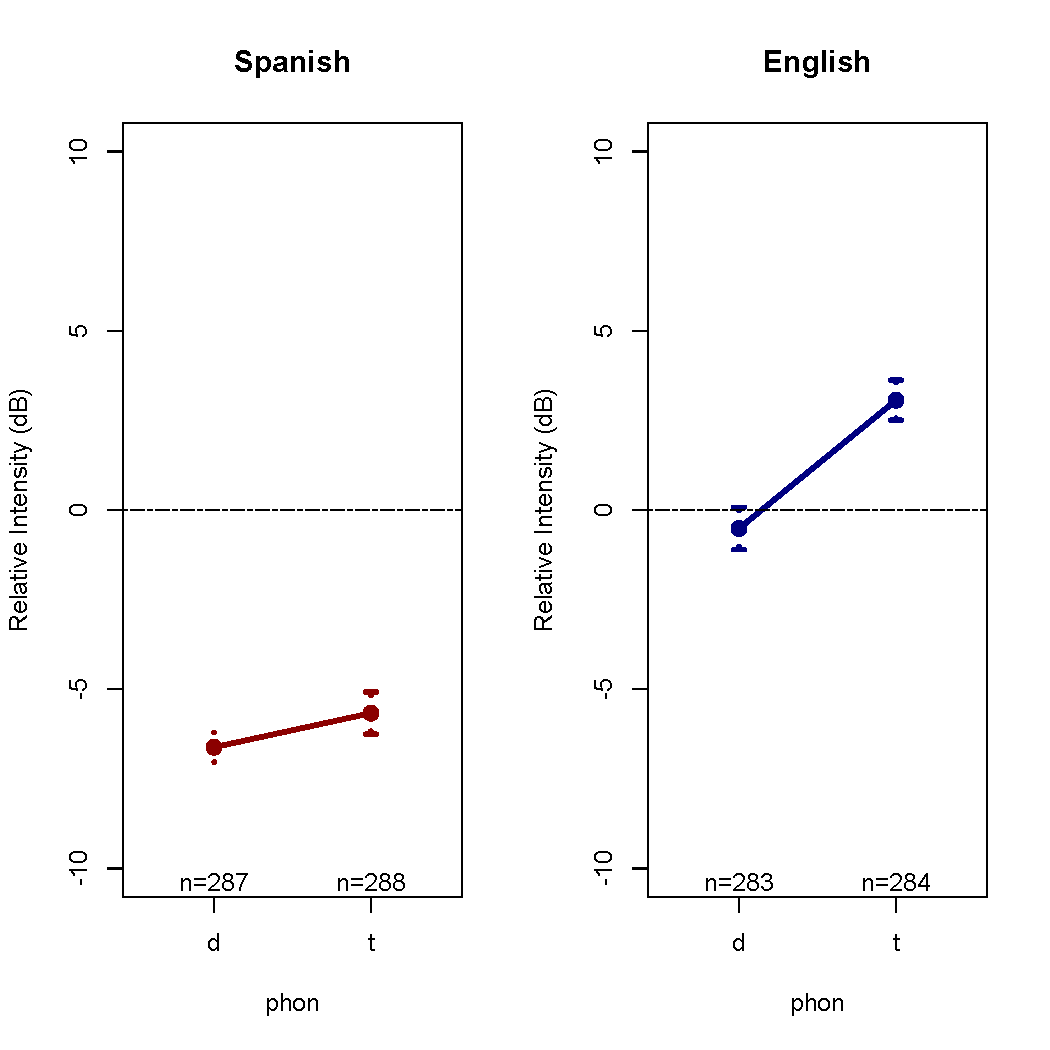
\includegraphics[scale=.375]{simplified/fig03_rimonolinguals.pdf}
\end{center}
\end{frame}

\begin{frame}
\frametitle{Summary of findings}
Spanish /d t/ differ from English /d t/...
\begin{center}
\begin{tabular}{l l l}
\cmark & VOT & (ms) \\
\cmark & Center of Gravity & (Hz) \\
\cmark & Relative Intensity & (dB) \\
\end{tabular}
\end{center}
\end{frame}

\subsection{Study 2: Spanish \textipa{/d t/} across groups}

\frame{\begin{center} \textbf{study 2} \\ Spanish \textipa{/d t/} across groups \end{center}}

\begin{frame}
\frametitle{Voice Onset Times (ms)}
\begin{center}
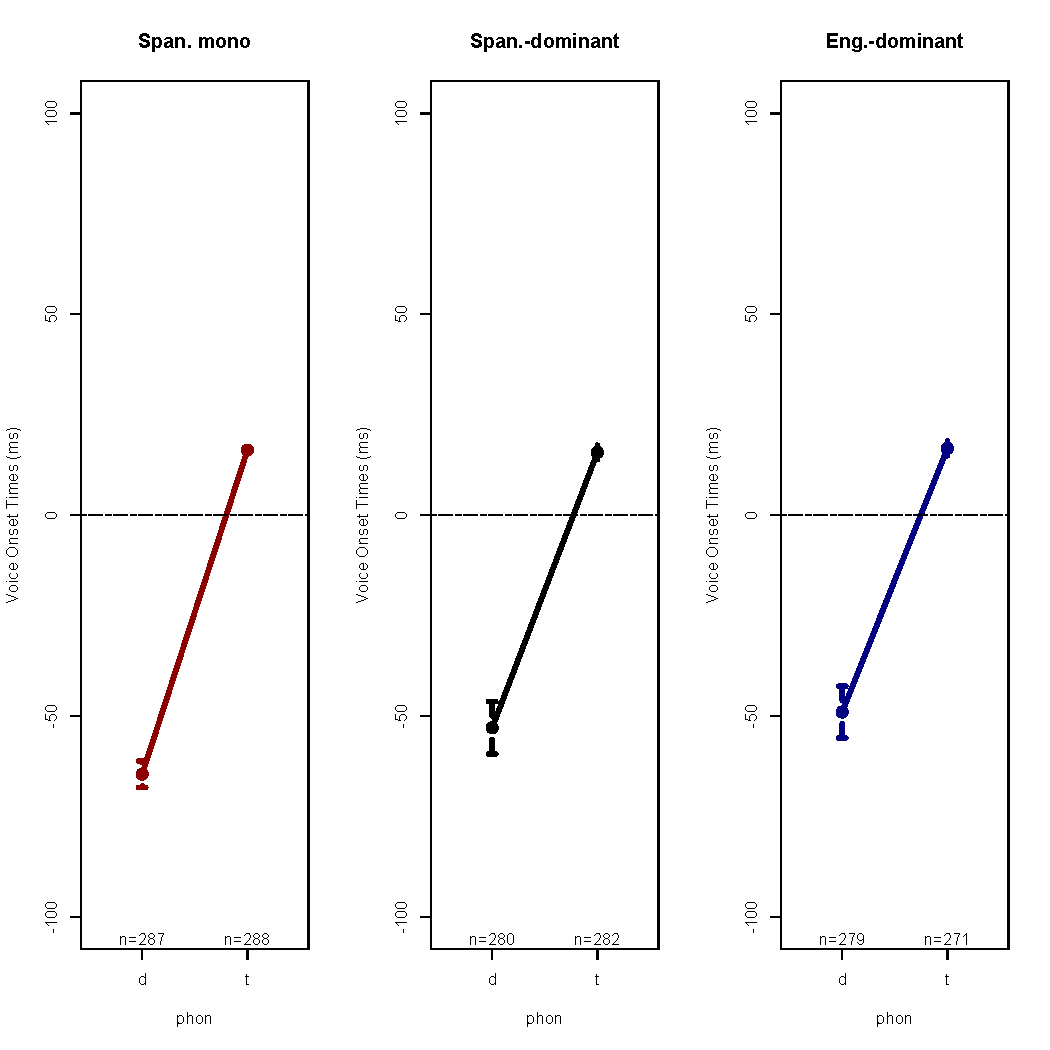
\includegraphics[scale=.375]{simplified/fig04_votspanish.pdf}
\end{center}
\end{frame}

\begin{frame}
\frametitle{Center of Gravity (Hz)}
\begin{center}
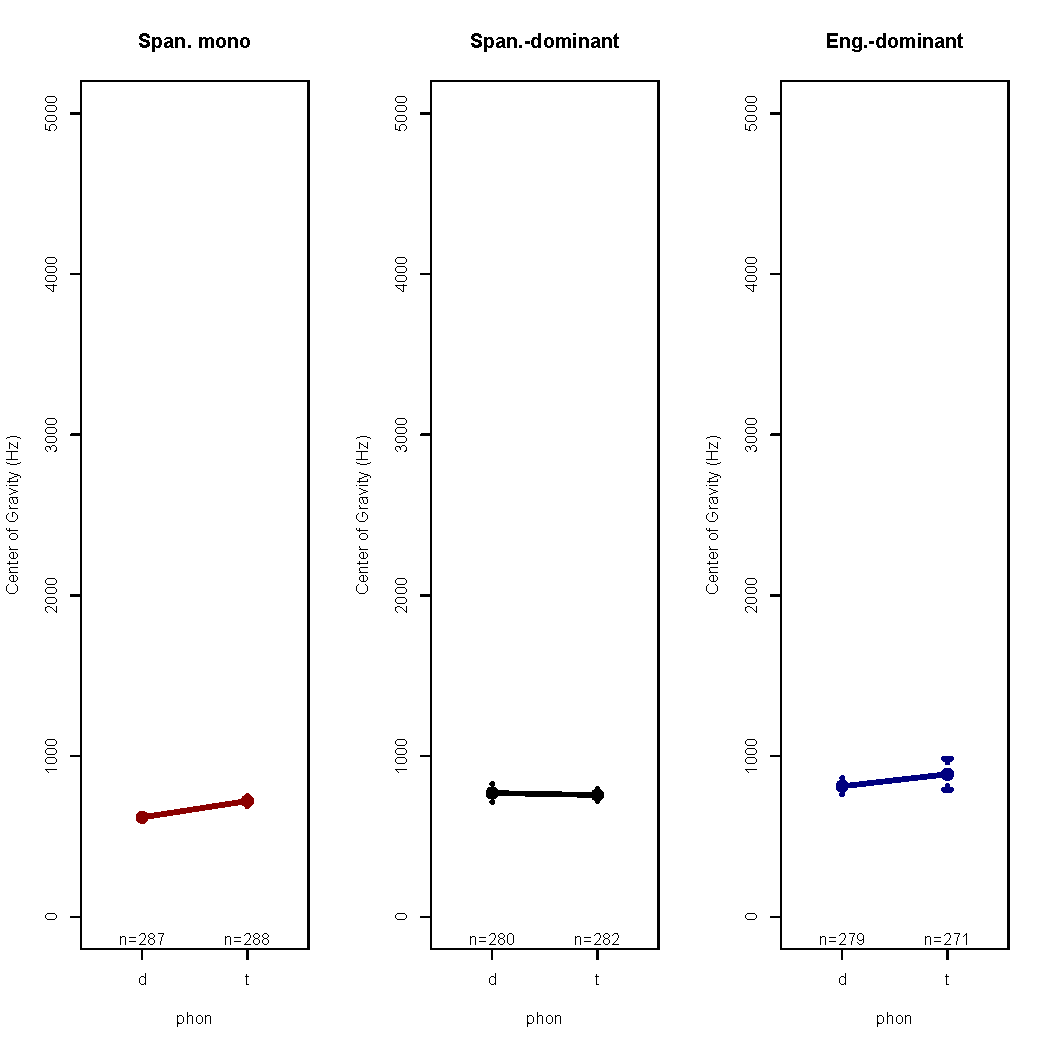
\includegraphics[scale=.375]{simplified/fig05_cogspanish.pdf}
\end{center}
\end{frame}

\begin{frame}
\frametitle{Relative Intensity (dB)}
\begin{center}
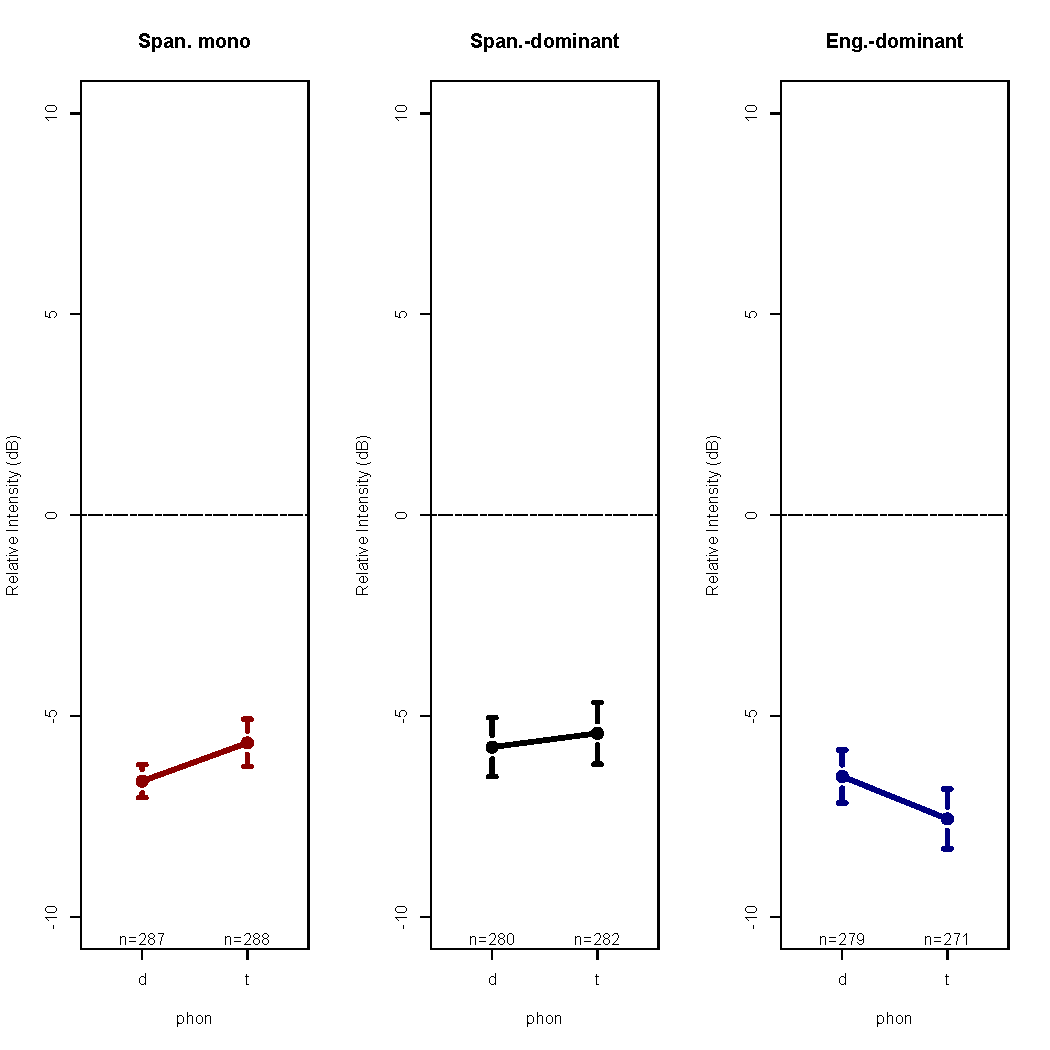
\includegraphics[scale=.375]{simplified/fig06_rispanish.pdf}
\end{center}
\end{frame}

\begin{frame}
\frametitle{Summary of findings}
Monolingual and bilingual Spanish speakers differ...
\begin{center}
\begin{tabular}{l l l}
\xmark & VOT & (ms) \\
\cmark & Center of Gravity & (Hz) \\
\xmark & Relative Intensity & (dB) \\
\end{tabular}
\end{center}
but effect size is tiny
\end{frame}

\subsection{Study 3: English \textipa{/d t/} across groups}

\frame{\begin{center} \textbf{study 3} \\ English \textipa{/d t/} across groups \end{center}}

\begin{frame}
\frametitle{Voice Onset Times (ms)}
\begin{center}
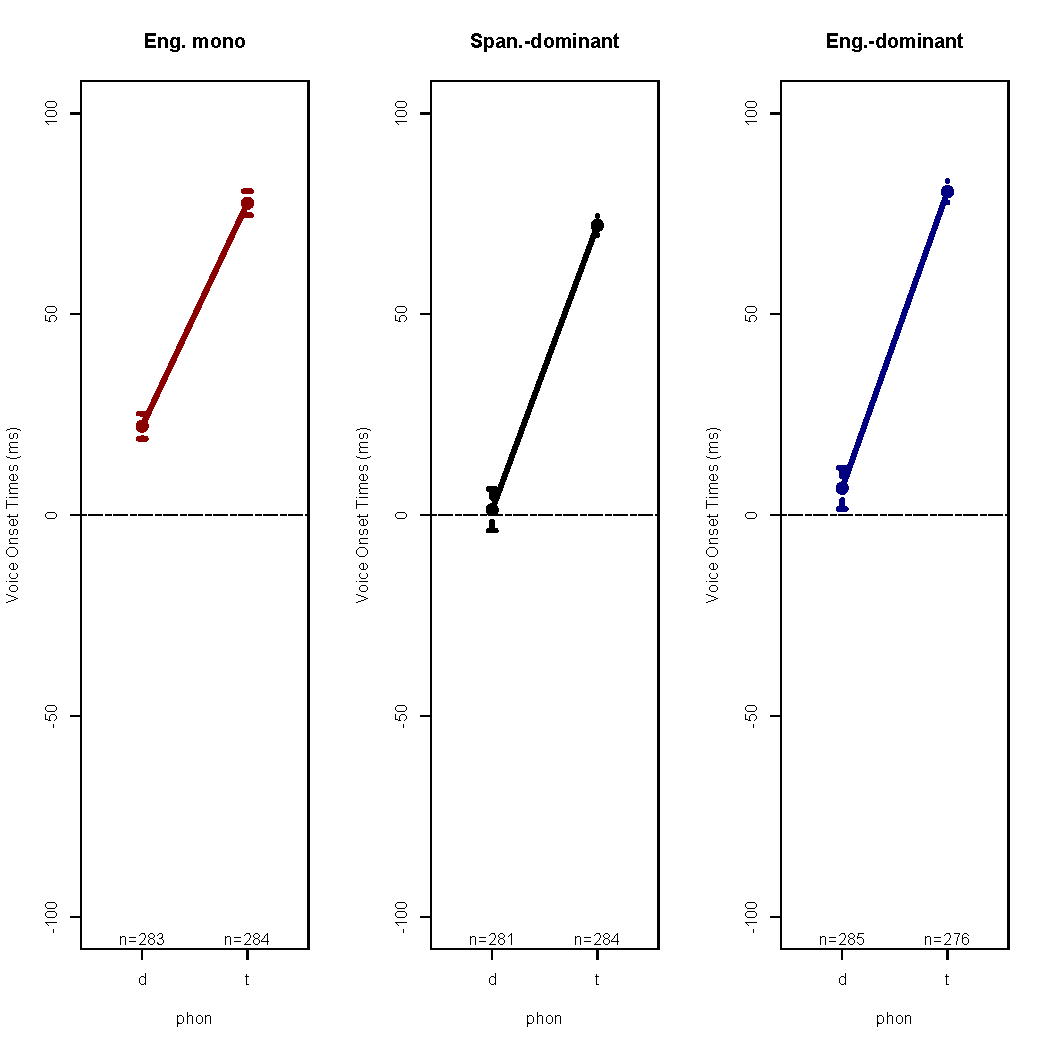
\includegraphics[scale=.375]{simplified/fig07_votenglish.pdf}
\end{center}
\end{frame}

\begin{frame}
\frametitle{Center of Gravity (Hz)}
\begin{center}
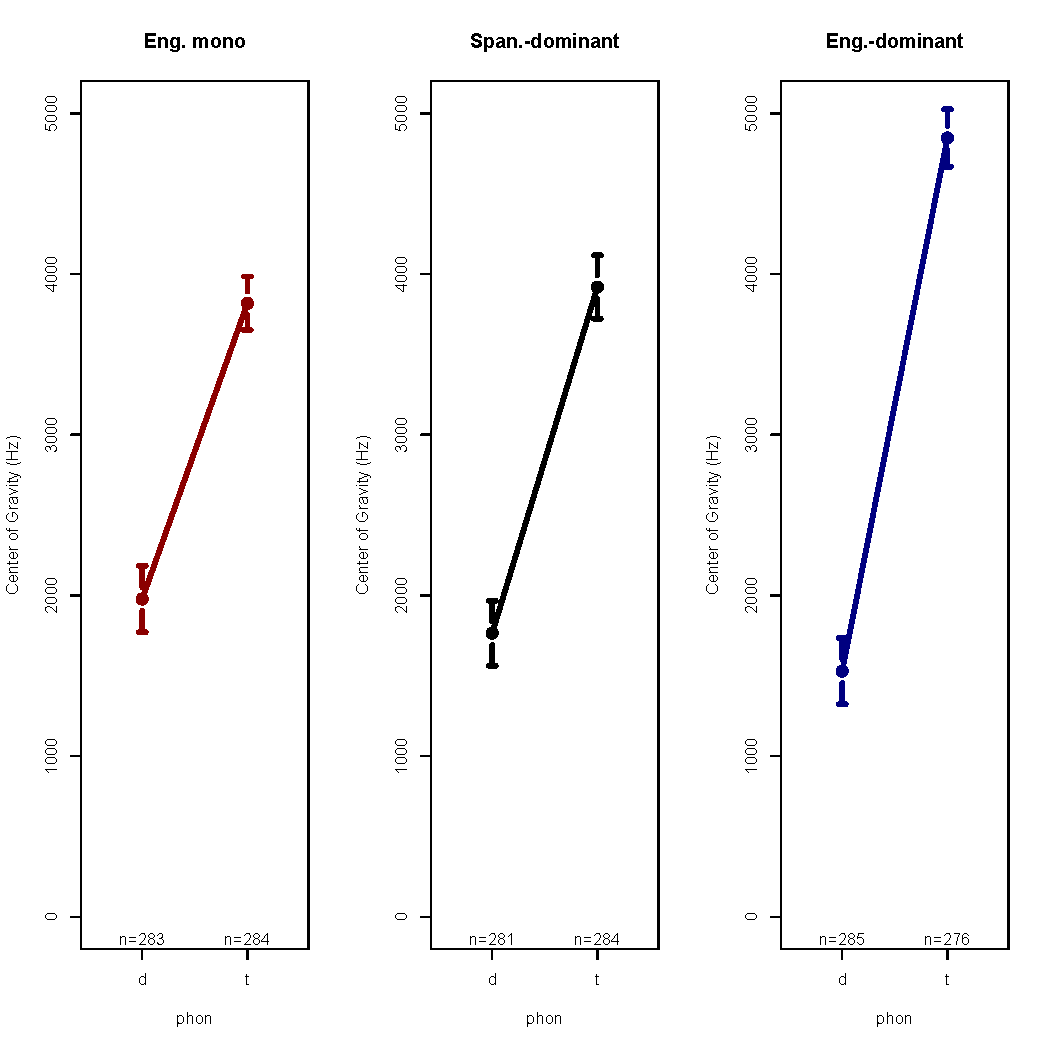
\includegraphics[scale=.375]{simplified/fig08_cogenglish.pdf}
\end{center}
\end{frame}

\begin{frame}
\frametitle{Relative Intensity (dB)}
\begin{center}
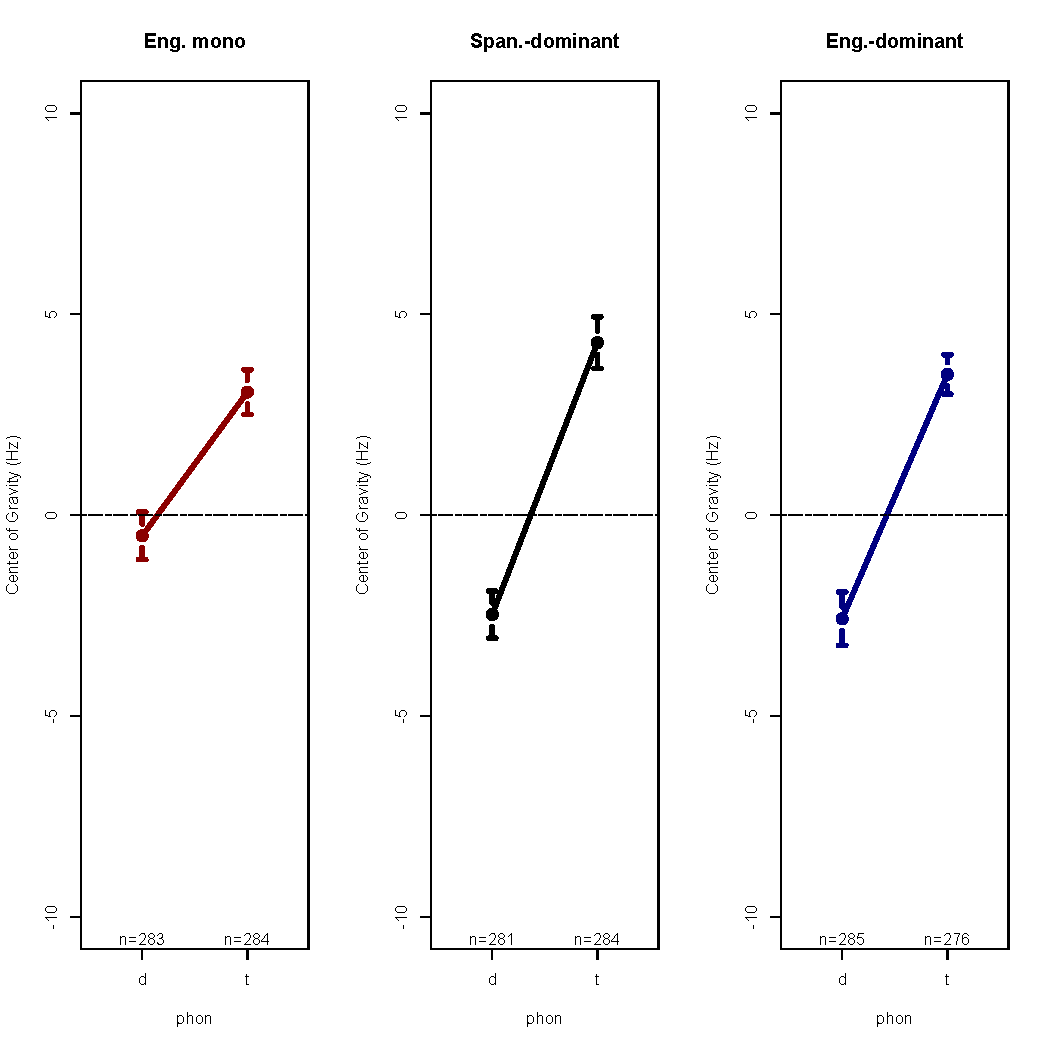
\includegraphics[scale=.375]{simplified/fig09_rienglish.pdf}
\end{center}
\end{frame}

\begin{frame}
\frametitle{Summary of findings}
Monolingual and bilingual Spanish speakers differ...
\begin{center}
\begin{tabular}{l l l}
\xmark & VOT & (ms) \\
\xmark & Center of Gravity & (Hz) \\
\xmark & Relative Intensity & (dB) \\
\end{tabular}
\end{center}
(perhaps) some tendencies for prevoicing in /d/ (in bilinguals) and higher-frequency resonances in /t/ (in bilinguals)
\end{frame}

\subsection{Study 4: Spanish vs. English \textipa{/d t/} in bilinguals}

\frame{\begin{center} \textbf{study 4} \\ Spanish vs. English \textipa{/d t/} in bilinguals \end{center}}

\begin{frame}
\frametitle{Voice Onset Times (ms)}
\begin{center}
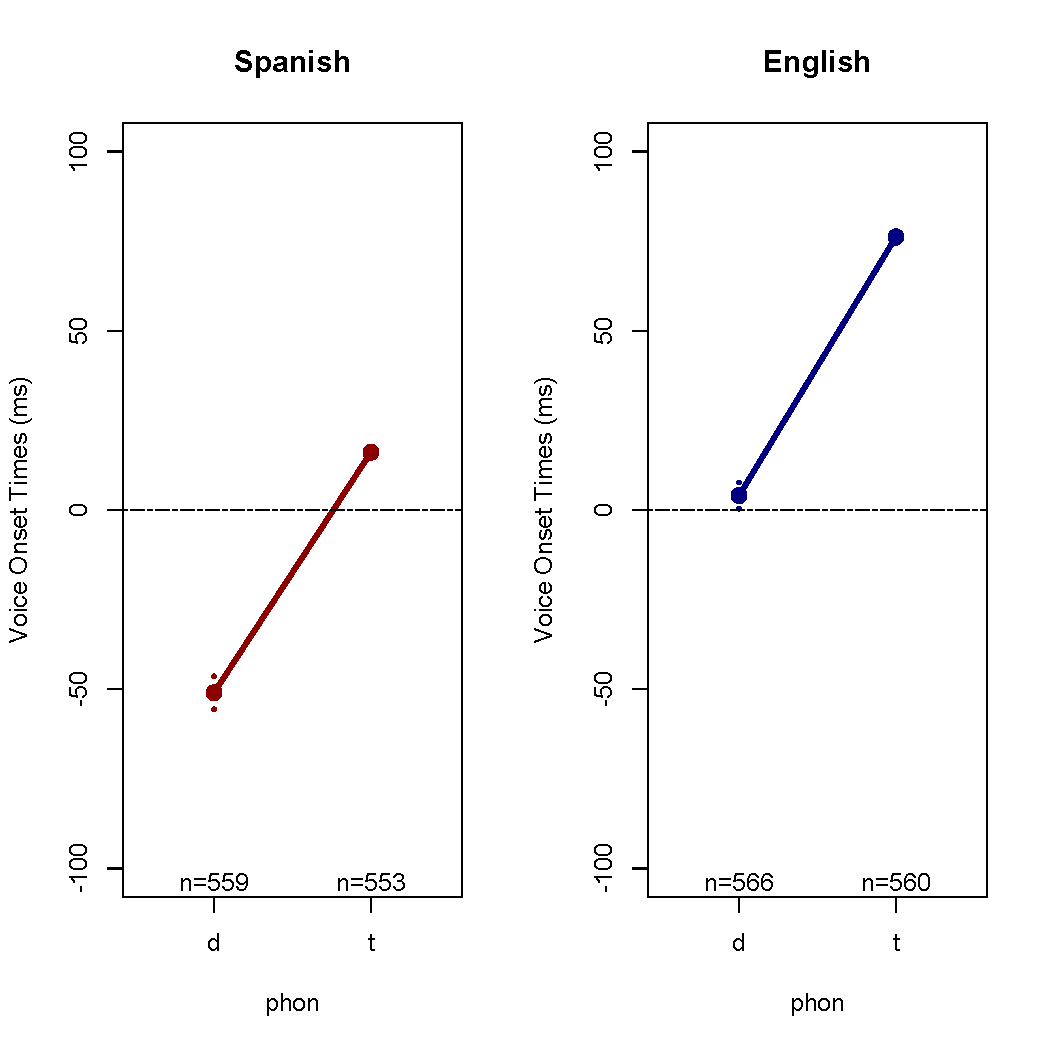
\includegraphics[scale=.375]{simplified/fig10_votbilinguals.pdf}
\end{center}
\end{frame}

\begin{frame}
\frametitle{Center of Gravity (Hz)}
\begin{center}
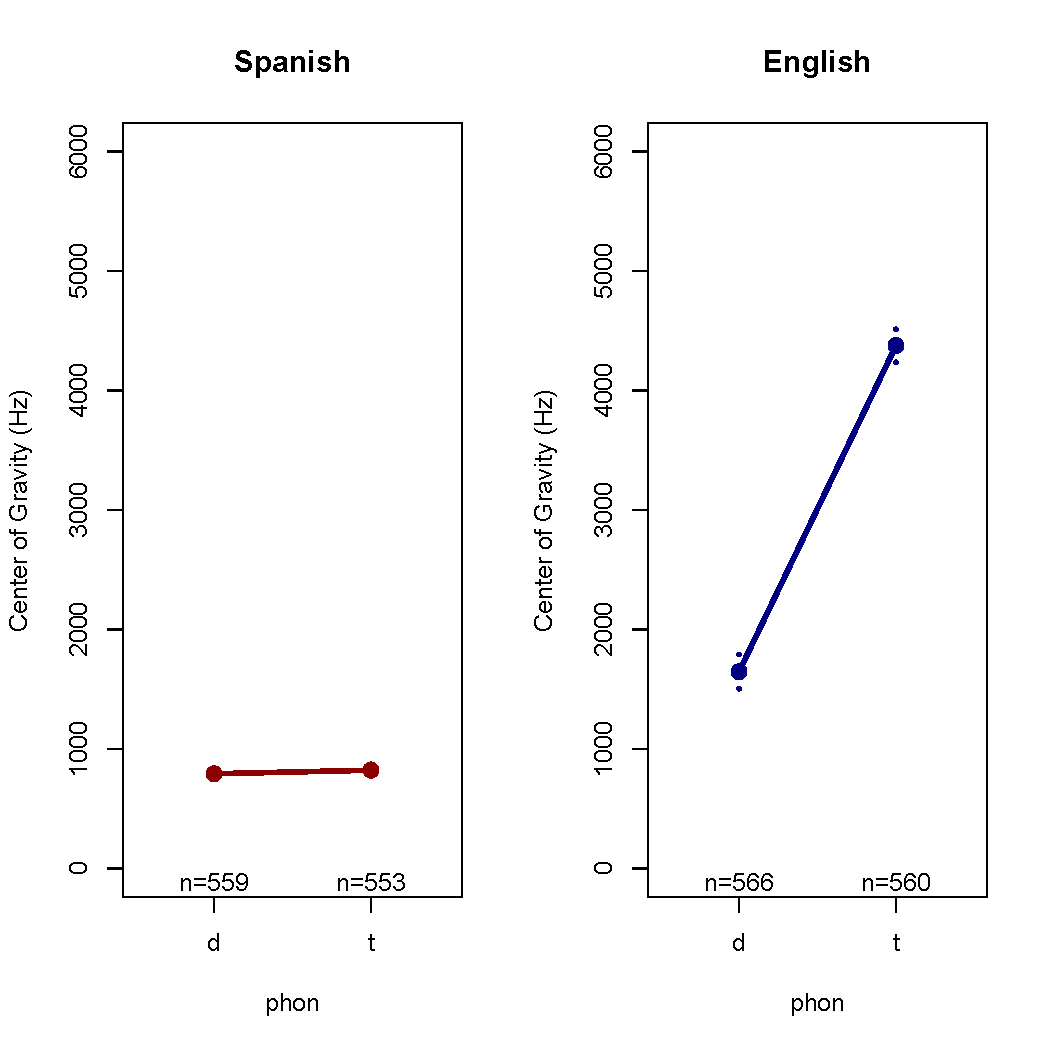
\includegraphics[scale=.375]{simplified/fig11_cogbilinguals.pdf}
\end{center}
\end{frame}

\begin{frame}
\frametitle{Relative Intensity (dB)}
\begin{center}
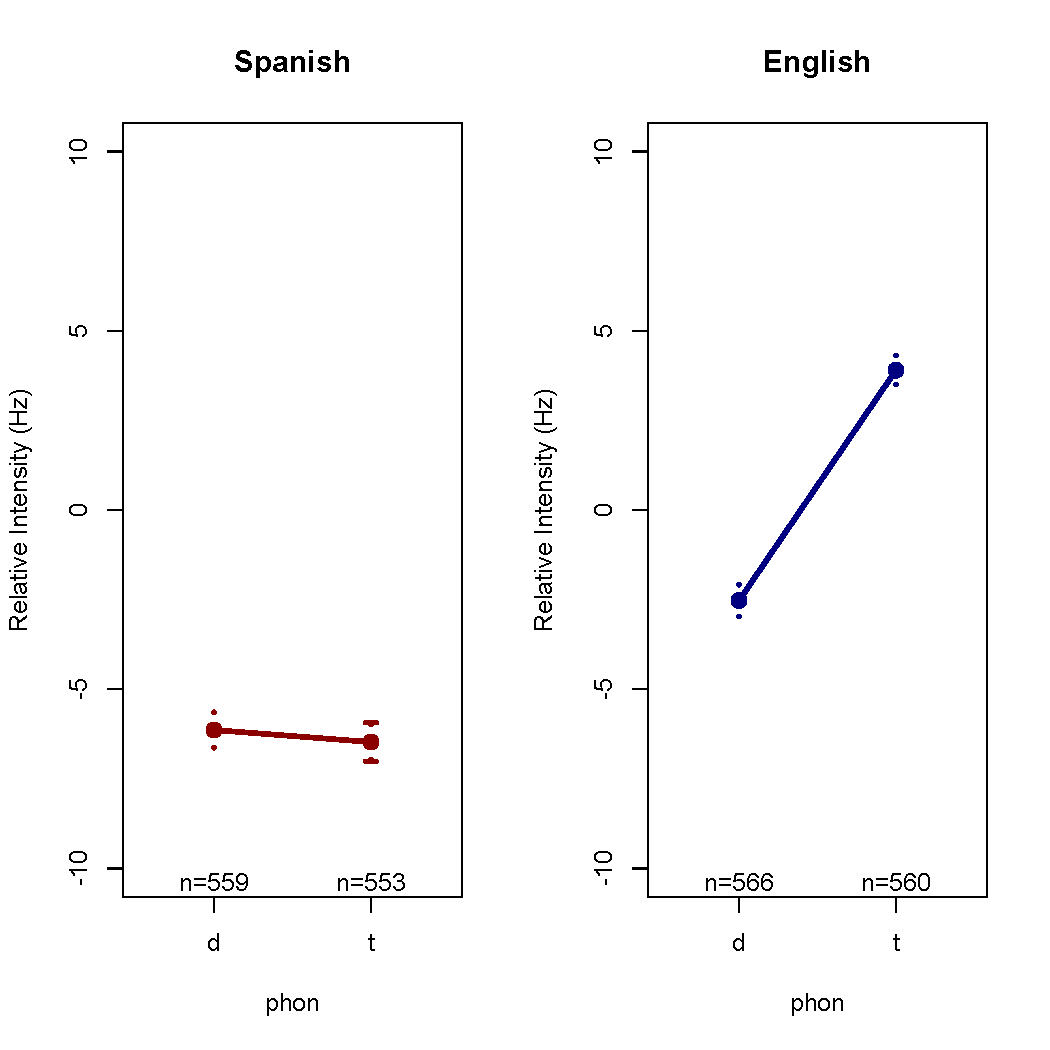
\includegraphics[scale=.375]{simplified/fig12_ribilinguals.pdf}
\end{center}
\end{frame}

\begin{frame}
\frametitle{Summary of findings}
English /d t/ differ from Spanish /d t/ in bilinguals in...
\begin{center}
\begin{tabular}{l l l}
\cmark & VOT & (ms) \\
\cmark & Center of Gravity & (Hz) \\
\cmark & Relative Intensity & (dB) \\
\end{tabular}
\end{center}
bilinguals keep separate (sub)systems
\end{frame}

\begin{frame}
\frametitle{The plot of all plots}
	\begin{figure}
		\centering
		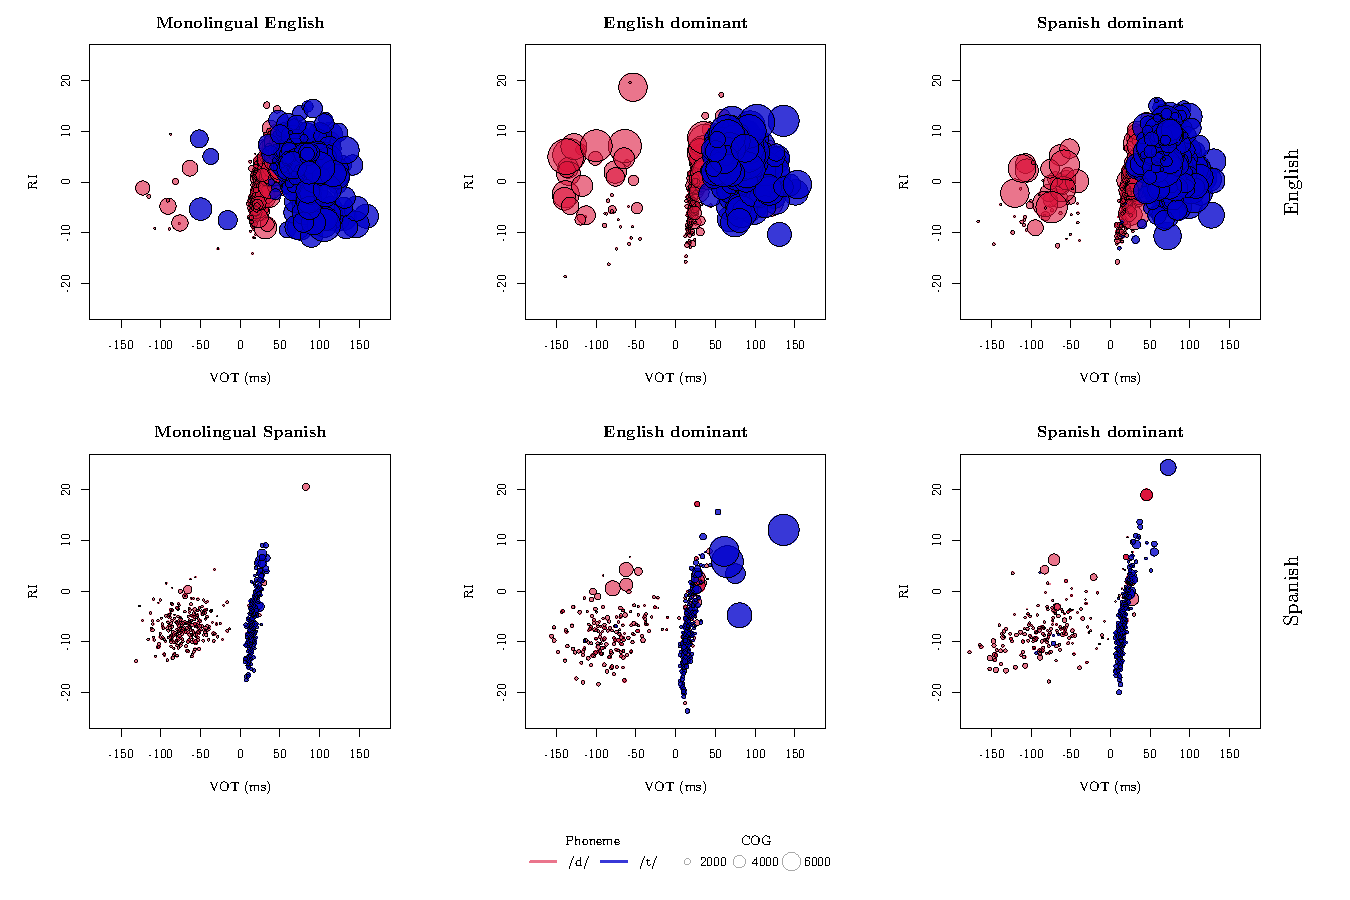
\includegraphics[scale=0.45]{figures/all.pdf}
	\end{figure}
\end{frame}

\section{Discussion}

\frame{\begin{center} \textbf{DISCUSSION} \\ summary | interpretation | conclusion \end{center}}

\subsection{Summary}

\begin{frame}
\frametitle{Findings}
\begin{itemize}
	\item \textbf{Spanish and English coronal stops (\textipa{/d t/}) differ \\ in their acoustic characteristics}
	\begin{itemize}
		\item differences in use of VOT for \emph{fortis-lenis} contrast
		\item differences in resonant frequencies at burst
		\item differences in amplitude of burst
	\end{itemize}
	\item \textbf{Spanish \textipa{/d t/}}
	\begin{itemize}
		\item have softer bursts with lower resonance frequencies
	\end{itemize}
	\item \textbf{English \textipa{/d t/}}
	\begin{itemize}
		\item have louder bursts with higher resonance frequencies
	\end{itemize}
\end{itemize}
\end{frame}

\begin{frame}
\frametitle{Findings}
\begin{itemize}
	\item \textbf{Spanish and English coronal stops (\textipa{/d t/}) differ \\ in their acoustic characteristics}
	\begin{itemize}
		\item differences hold across across individuals (languages) when monolingual speakers are compared
		\item and they hold within individuals when \\ bilingual speakers are compared
	\end{itemize}
	\item bilinguals differ from monolinguals only very slightly
	\item \textbf{bilinguals have separate (sub)systems \\ for stops in their two languages}
\end{itemize}
\end{frame}

\subsection{Interpretation}

\begin{frame}
\frametitle{Context}
\textbf{Findings in line with...}
\begin{itemize}
	\item Jongman et al. (1985) \begin{itemize} \item for Malayalam, which contrasts dental and alveolar stops, and Dutch (dental) vs. English (alveolar) stops \end{itemize}
	\item Stoel-Gamon et al. (1994) \begin{itemize} \item for Swedish (dental) vs. English (alveolar) stops \end{itemize}
	\item Sundara (2005, 2006) \begin{itemize} \item for Canadian French and Canadian English \\ and French-English bilinguals\end{itemize}
	\item Spanish \textipa{/d t/} pattern with French, Dutch and Swedish \\ \alert{Spanish \textipa{/d t/} are (probably) dental or laminal}
\end{itemize}
\end{frame}

\begin{frame}
\frametitle{Acoustics and articulation}
\begin{itemize}
	\item \textbf{burst amplitude differences}
	\begin{itemize}
		\item perhaps laminal (dental) constrictions, which have more contact surface, are released more slowly than apical (alveolar) constrictions
		\item perhaps path of airstrem after constriction differs and it hits more of an obstacle (teeth) in alveolars than in dentals
	\end{itemize}
	\item resonance frequencies
	\begin{itemize}
		\item if dental contact is more fronted than alveolar contact, we expect higher resonance frequencies for dentals because the size of the front cavity would be smaller for dentals
		\item not the obtained pattern (pattern is consistently reversed)
		\item at release, there must not be a difference in fronting of constriction
	\end{itemize}
\end{itemize}
\end{frame}

\begin{frame}
\frametitle{Acoustics and articulation}
\begin{itemize}
	\item burst amplitude differences
	\begin{itemize}
		\item perhaps laminal (dental) constrictions, which have more contact surface, are released more slowly than apical (alveolar) constrictions
		\item perhaps path of airstrem after constriction differs and it hits more of an obstacle (teeth) in alveolars than in dentals
	\end{itemize}
	\item \textbf{resonance frequencies}
	\begin{itemize}
		\item if dental contact is more fronted than alveolar contact, we expect higher resonance frequencies for dentals, because the size of the front cavity would be smaller for dentals
		\item not the obtained pattern (pattern is consistently reversed)
		\item at release, there must not be a difference in fronting of constriction
	\end{itemize}
\end{itemize}
\end{frame}

\subsection{Conclusion}

\begin{frame}
\frametitle{Conclusion}
\begin{itemize}
	\item \textbf{Acoustics of Spanish and English coronal stops differ}
	\begin{itemize}
		\item attested differences in line with prior descriptions of \\ dental vs. alveolar stops, within and across languages
		\item articulatory-acoustic link continues to be a mistery
	\end{itemize}
	\item \textbf{Early, proficient Spanish-English bilinguals from Arizona keep separate (sub)systems for their coronal consonants}
	\begin{itemize}
		\item sometimes \emph{the bilingual is two monolinguals in one person}\footnote{Grosjean, 1989}
	\end{itemize}
\end{itemize}
\end{frame}


\begin{frame}
\frametitle{Thank you}
\begin{tabular}{l r c l}
\textbf{Joseph V. Casillas} & jvcasill &@ & email.arizona.edu \\ 
\textbf{Yamile D\'{i}az} & ydiaz44 & @ & email.arizona.edu \\
\textbf{Miquel Simonet} & simonet &@ &email.arizona.edu\\
\end{tabular}
\begin{center}

\includegraphics[scale=.75]{aalp_logo.pdf}
\end{center}
\end{frame}

\end{document}




